\documentclass[norsk,11pt,a4paper]{report}
\usepackage[margin=1cm,tmargin=1cm,bmargin=1cm,rmargin=1in,lmargin=1in,footskip=.2in]{geometry}
\title{REAL112-1 24H - Matematikk\\Obligatorisk innlevering 6}
\author{Casper Eide Özdemir-Børretzen}
\date{}

% % % % % % % % % % % % % % % % % % % % % % % % % % % % % % % % % % % % % % % % 

\usepackage{babel}               % Support for other languages than english
\usepackage{setspace}            % Set paragraph spacing
\usepackage{nicefrac}            % Nice looking fractals
\usepackage{graphicx}            % Images
\usepackage{gensymb}             % Degree symbol
\usepackage{listings}            % Code
\usepackage{ulem}                % Double underline
\usepackage{amssymb}             % ...
\usepackage{pdfpages}            % Insert pdf pages
\usepackage{enumitem}            % Lists
\usepackage{titlesec}            % ...
\usepackage[T1]{fontenc}         % ...
\usepackage[utf8]{inputenc}      % ...
\usepackage[fleqn]{amsmath}      % ...
\usepackage[makeroom]{cancel}    % ...
%\usepackage{empheq}              % ...
\setstretch{1.5}
\setlength{\parindent}{0pt}
\titlespacing*{\subsection}{0cm}{2cm}{0.5cm}
\lstset{
aboveskip=0cm,
belowskip=0cm,
showstringspaces=false,
columns=flexible,
basicstyle={\scriptsize\ttfamily},
breaklines=true,
breakatwhitespace=true,
tabsize=4,
inputencoding = utf8,  % Input encoding
extendedchars = true,  % Extended ASCII
literate      =        % Support additional characters
{á}{{\'a}}1  {é}{{\'e}}1  {í}{{\'i}}1 {ó}{{\'o}}1  {ú}{{\'u}}1
{Á}{{\'A}}1  {É}{{\'E}}1  {Í}{{\'I}}1 {Ó}{{\'O}}1  {Ú}{{\'U}}1
{à}{{\`a}}1  {è}{{\`e}}1  {ì}{{\`i}}1 {ò}{{\`o}}1  {ù}{{\`u}}1
{À}{{\`A}}1  {È}{{\`E}}1  {Ì}{{\`I}}1 {Ò}{{\`O}}1  {Ù}{{\`U}}1
{ä}{{\"a}}1  {ë}{{\"e}}1  {ï}{{\"i}}1 {ö}{{\"o}}1  {ü}{{\"u}}1
{Ä}{{\"A}}1  {Ë}{{\"E}}1  {Ï}{{\"I}}1 {Ö}{{\"O}}1  {Ü}{{\"U}}1
{â}{{\^a}}1  {ê}{{\^e}}1  {î}{{\^i}}1 {ô}{{\^o}}1  {û}{{\^u}}1
{Â}{{\^A}}1  {Ê}{{\^E}}1  {Î}{{\^I}}1 {Ô}{{\^O}}1  {Û}{{\^U}}1
{œ}{{\oe}}1  {Œ}{{\OE}}1  {æ}{{\ae}}1 {Æ}{{\AE}}1  {ß}{{\ss}}1
{ẞ}{{\SS}}1  {ç}{{\c{c}}}1 {Ç}{{\c{C}}}1 {ø}{{\o}}1  {Ø}{{\O}}1
{å}{{\aa}}1  {Å}{{\AA}}1  {ã}{{\~a}}1  {õ}{{\~o}}1 {Ã}{{\~A}}1
{Õ}{{\~O}}1  {ñ}{{\~n}}1  {Ñ}{{\~N}}1  {¿}{{?`}}1  {¡}{{!`}}1
{„}{\quotedblbase}1 {“}{\textquotedblleft}1 {–}{$-$}1
{°}{{\textdegree}}1 {º}{{\textordmasculine}}1 {ª}{{\textordfeminine}}1
{£}{{\pounds}}1  {©}{{\copyright}}1  {®}{{\textregistered}}1
{«}{{\guillemotleft}}1  {»}{{\guillemotright}}1  {Ð}{{\DH}}1  {ð}{{\dh}}1
{Ý}{{\'Y}}1    {ý}{{\'y}}1    {Þ}{{\TH}}1    {þ}{{\th}}1    {Ă}{{\u{A}}}1
{ă}{{\u{a}}}1  {Ą}{{\k{A}}}1  {ą}{{\k{a}}}1  {Ć}{{\'C}}1    {ć}{{\'c}}1
{Č}{{\v{C}}}1  {č}{{\v{c}}}1  {Ď}{{\v{D}}}1  {ď}{{\v{d}}}1  {Đ}{{\DJ}}1
{đ}{{\dj}}1    {Ė}{{\.{E}}}1  {ė}{{\.{e}}}1  {Ę}{{\k{E}}}1  {ę}{{\k{e}}}1
{Ě}{{\v{E}}}1  {ě}{{\v{e}}}1  {Ğ}{{\u{G}}}1  {ğ}{{\u{g}}}1  {Ĩ}{{\~I}}1
{ĩ}{{\~\i}}1   {Į}{{\k{I}}}1  {į}{{\k{i}}}1  {İ}{{\.{I}}}1  {ı}{{\i}}1
{Ĺ}{{\'L}}1    {ĺ}{{\'l}}1    {Ľ}{{\v{L}}}1  {ľ}{{\v{l}}}1  {Ł}{{\L{}}}1
{ł}{{\l{}}}1   {Ń}{{\'N}}1    {ń}{{\'n}}1    {Ň}{{\v{N}}}1  {ň}{{\v{n}}}1
{Ő}{{\H{O}}}1  {ő}{{\H{o}}}1  {Ŕ}{{\'{R}}}1  {ŕ}{{\'{r}}}1  {Ř}{{\v{R}}}1
{ř}{{\v{r}}}1  {Ś}{{\'S}}1    {ś}{{\'s}}1    {Ş}{{\c{S}}}1  {ş}{{\c{s}}}1
{Š}{{\v{S}}}1  {š}{{\v{s}}}1  {Ť}{{\v{T}}}1  {ť}{{\v{t}}}1  {Ũ}{{\~U}}1
{ũ}{{\~u}}1    {Ū}{{\={U}}}1  {ū}{{\={u}}}1  {Ů}{{\r{U}}}1  {ů}{{\r{u}}}1
{Ű}{{\H{U}}}1  {ű}{{\H{u}}}1  {Ų}{{\k{U}}}1  {ų}{{\k{u}}}1  {Ź}{{\'Z}}1
{ź}{{\'z}}1    {Ż}{{\.Z}}1    {ż}{{\.z}}1    {Ž}{{\v{Z}}}1  {ž}{{\v{z}}}1
}

% % % % % % % % % % % % % % % % % % % % % % % % % % % % % % % % % % % % % % % % 

%\newcommand{\enkelsvaralign}[1]{\makebox[0pt][l]{\uuline{\phantom{$#1$}}}#1}
%\newcommand{\svaralign}[2]{\makebox[0pt][l]{\uuline{\phantom{$#1 #2$}}}#1 &#2}
\newcommand{\oppgave}[1]{\subsection*{Oppgave #1}}
\newcommand{\oppgaveDelStart}{\begin{enumerate}[leftmargin=*,itemsep=1cm,labelsep=1.5em,label=\alph*)]}
\newcommand{\oppgaveDelSlutt}{\end{enumerate}}
\newcommand{\oppgaveDel}[1]{\item[#1)]}
\newcommand{\m}{\cdot}

% % % % % % % % % % % % % % % % % % % % % % % % % % % % % % % % % % % % % % % % 

\begin{document}
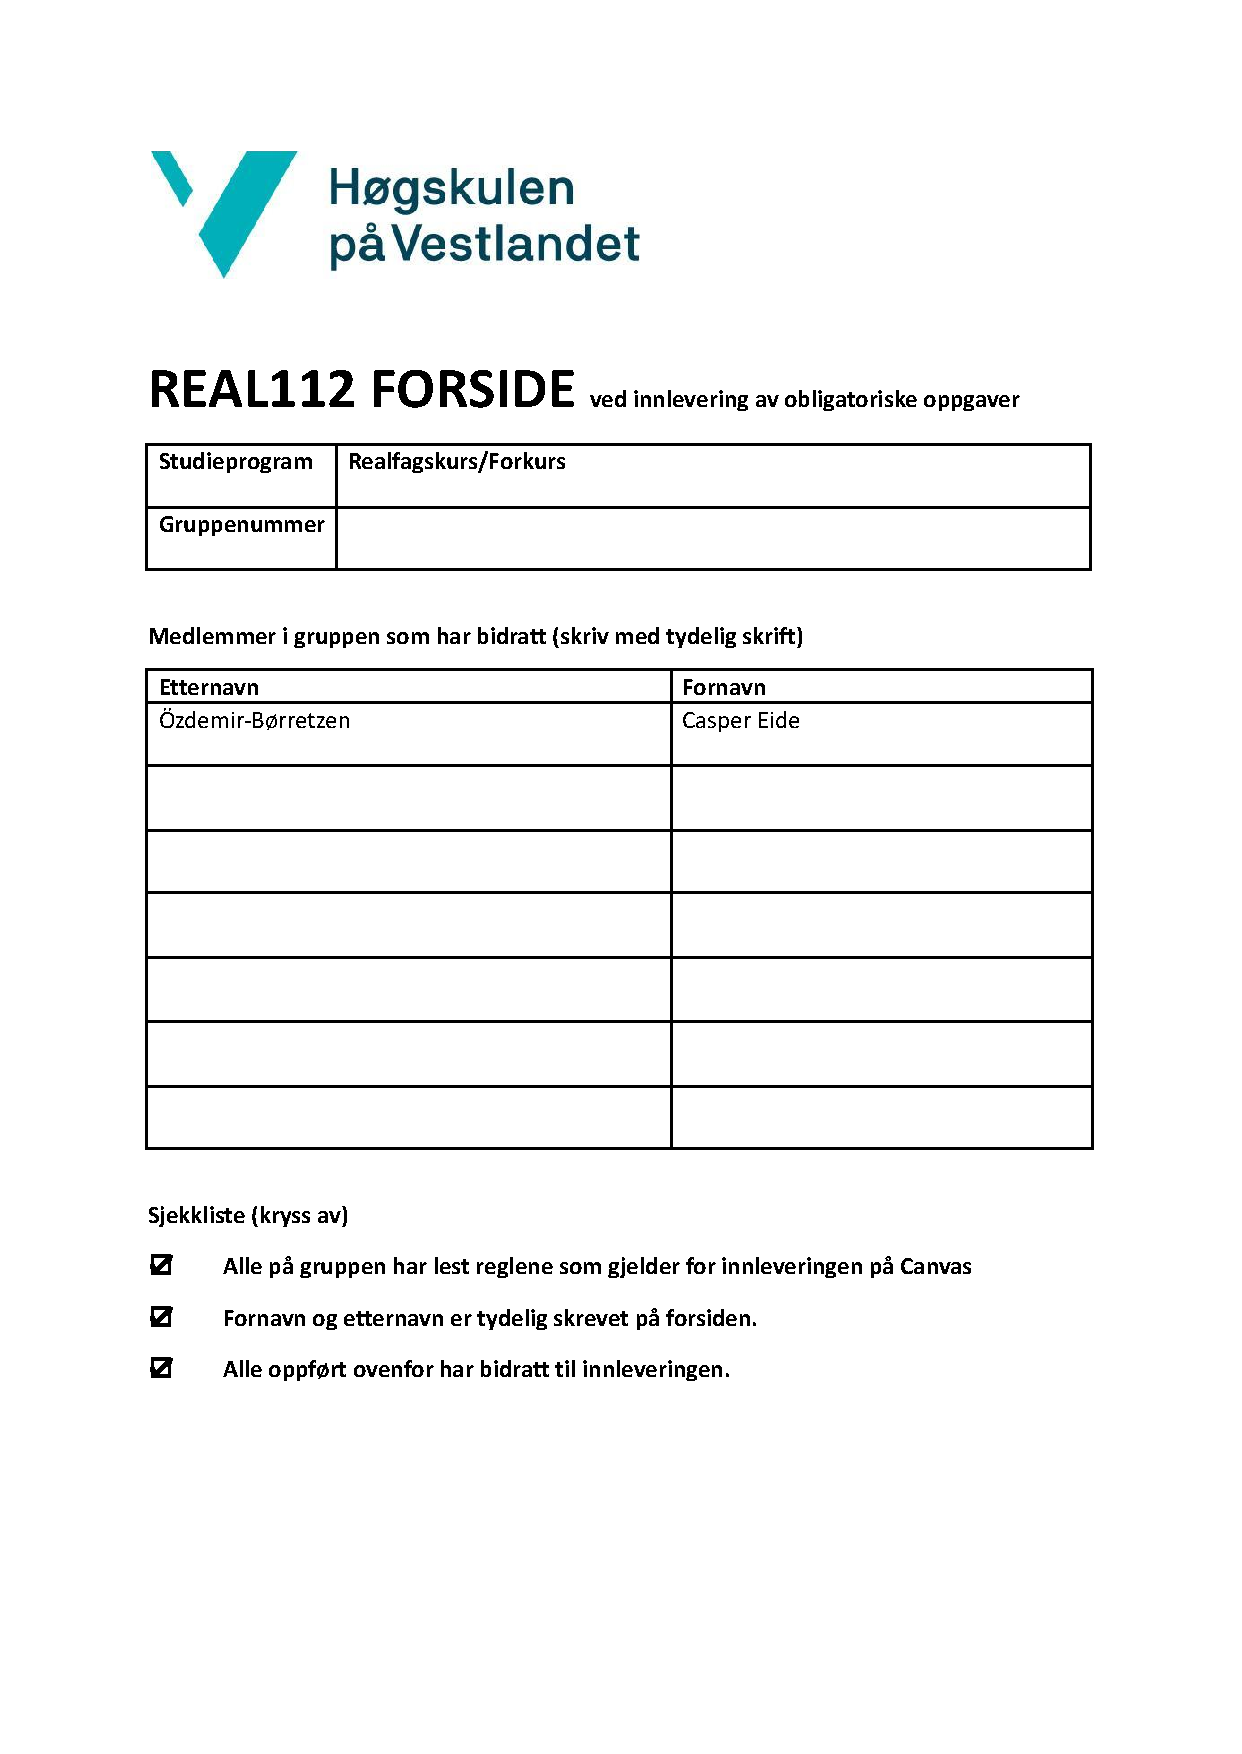
\includepdf[pages={1}]{real112-forside.pdf}

% % % % % % % % % % % % % % % % % % % % % % % % % % % % % % % % % % % % % % % % 

\oppgave{1}
\begin{align*}
&\vec{v} = [1, 2, 3]\\
&\vec{u} = [3, 2, 1]\\
\end{align*}
\oppgaveDelStart
\oppgaveDel{a}
\begin{align*}
&|\vec{v}| = \sqrt{1^2 + 2^2 + 3^2} = \sqrt{1 + 4 + 9} = \uuline{\sqrt{14}}\\
&|\vec{u}| = \sqrt{3^2 + 2^2 + 1^2} = \sqrt{9 + 4 + 1} = \uuline{\sqrt{14}}\\
&|\vec{v}| = |\vec{u}|
\end{align*}

\oppgaveDel{b}
\begin{align*}
&\vec{v} \m \vec{u} = 1 \m 3 + 2 \m 2 + 3 \m 1 = 3 + 4 + 3 = 10\\
&\vec{v} \m \vec{u} = |\vec{v}| \m |\vec{u}| \m \cos u\\
&u = cos^{-1} \left( \frac{\vec{v} \m \vec{u}}{|\vec{v}| \m |\vec{u}|} \right) = cos^{-1} \left( \frac{10}{\sqrt{14 \m 14}} \right) = 44,42 \degree\\
&\angle{(\vec{u}, \vec{v})} = \uuline{44,42 \degree}
\end{align*}

\oppgaveDel{c}
Likningen for plan gjennom $[0, 0, 0]$ med normalvektor $\vec{v}$ er:\\
$x + 2y + 3z = 0$\\\\
Likningen for plan gjennom $[0, 0, 0]$ med normalvektor $\vec{u}$ er:\\
$3x + 2y + z = 0$

\newpage
\oppgaveDel{d}
\begin{align*}
&\vec{v} \times \vec{u} = 
\begin{vmatrix}
\vec{e_1} & \vec{e_2} & \vec{e_3}\\
1 & 2 & 3\\
3 & 2 & 1
\end{vmatrix}
=
\left[\ 
\begin{vmatrix}
2 & 3\\
2 & 1
\end{vmatrix}
\ ,\ -
\begin{vmatrix}
1 & 3\\
3 & 1
\end{vmatrix}
\ ,\ 
\begin{vmatrix}
1 & 2\\
3 & 2
\end{vmatrix}
\ \right]\\[0.2cm]
&\vec{v} \times \vec{u} = [2 \m 1 - 3 \m 2,\ -(1 \m 1 - 3\m 3),\ 1 \m 2 - 2 \m 3] = [2 - 6,\ -1 + 9,\ 2 - 6]\\
&\vec{v} \times \vec{u} = \uuline{[-4,8,-4]}
\end{align*}

\oppgaveDel{e}
Parameterfremstilling for plan gjennom $[0,0,0]$ med normalvektor $\vec{v}$:\\

\begin{equation*}
p_v:\begin{cases}
x=t\\
y=2t\\
z=3t
\end{cases}
\end{equation*}

Parameterfremstilling for plan gjennom $[0,0,0]$ med normalvektor $\vec{u}$:
\begin{equation*}
p_u:\begin{cases}
x=3t\\
y=2t\\
z=t
\end{cases}
\end{equation*}

\oppgaveDel{f}
\begin{align*}
&\text{(kryssprodukt hentet fra oppgave 1d)}\\
%&\vec{v} \times \vec{u} = [-4,8,-4]\\
&\vec{v} \times \vec{u} \m \frac{1}{4}= [-\frac{4}{4},\frac{8}{4},-\frac{4}{4}] = [-1,2,-1]\\[0.2cm]
&l:\begin{cases}x=-t\\y=2t\\z=-t\end{cases}
\end{align*}

\oppgaveDel{g}
\begin{align*}
&\vec{w} = [1,0,1]\\[0.2cm]
&\boxed{V = \frac{1}{3} \m D}\\[0.2cm]
&\text{Determinanten til $\vec{u}$, $\vec{v}$ og $\vec{w}$ er:}\\[0.2cm]
&D = \begin{vmatrix}3 & 2 & 1\\1 & 2 & 3\\ 1 & 0 & 1\end{vmatrix} = 3 \m \begin{vmatrix}2 & 3\\0 & 1\end{vmatrix} -2 \m \begin{vmatrix}1 & 3\\1 & 1\end{vmatrix} + 1 \m \begin{vmatrix}1 & 2\\1 & 0\end{vmatrix}\\[0.2cm]
&D = 3 \m (2 \m 1 - 3 \m 0) - 2 \m (1 \m 1 - 3 \m 1) + 1 \m (1 \m 0 - 2 \m 1) = 6 + 4 - 2 = 8\\[0.2cm]
&V = \frac{1}{3} \m D = \frac{1}{3} \m 8\\[0.2cm]
&V = \uuline{\frac{8}{3}}\\\\
&\text{Oppgaven kan også løses på denne måten:}\\
&\boxed{V = \frac{1}{3} \m \left|\ ( \vec{a} \times \vec{b}) \m \vec{c}\ \right|}\\[0.2cm]
&V = \frac{1}{3} \m \left|\ (\vec{u} \times \vec{v}) \m \vec{w}\ \right|\\[0.2cm]
&V = \frac{1}{3} \m \left|\ [-4,8-4] \m [1,0,1]\ \right| = \frac{1}{3} \m \left|\ ((-4) \m 1 + 8 \m 0 + (-4) \m 1) \right| = \frac{1}{3} \m |-8|\\[0.2cm]
&V = \uuline{\frac{8}{3}}
\end{align*}
\oppgaveDelSlutt

% % % % % % % % % % % % % % % % % % % % % % % % % % % % % % % % % % % % % % % % 

\oppgave{2}
\oppgaveDelStart
\oppgaveDel{a} $\int 2xdx = \uuline{x^2 + C}$
\oppgaveDel{b} $\int 2e^tdt = \uuline{2e^t + C}$
\oppgaveDel{c} $\int 2t \m e^{t^2}dt = \uuline{e^{t^2} + C}$
\oppgaveDelSlutt

% % % % % % % % % % % % % % % % % % % % % % % % % % % % % % % % % % % % % % % % 

\oppgave{3}
\oppgaveDelStart
\oppgaveDel{a} \begin{align*}&\int_{0}^{2} e^x dx = [e^x]_{0}^{2} = e^2 - e^0 = 7,39 - 1 = \uuline{6,39}\end{align*}
\oppgaveDel{b} \begin{align*}&\int_{0}^{\pi} \sin (2x) dx = \left[ \frac{-cos(2x)}{2} \right]_{0}^{\pi} = \frac{-cos(2\pi) - (-cos(0))}{2} = \frac{-1 + 1}{2} = \uuline{0}\end{align*}
\oppgaveDel{c}
\begin{align*}
&\int_{-\sqrt{1-\frac{1}{\pi}}}^{\ \ \sqrt{1-\frac{1}{\pi}}} 2 \pi x \m \sin (2 \pi x^2 + 1) dx\\[0.2cm]
&= \left[ \frac{\cancel{2 \pi x} \m (-\cos(\pi x^2 + 1))}{\cancel{2 \pi x}} \right]_{-\sqrt{1-\frac{1}{\pi}}}^{\ \ \sqrt{1-\frac{1}{\pi}}}\\[0.2cm]
&= \left[ -\cos(\pi x^2 + 1) \right]_{-\sqrt{1-\frac{1}{\pi}}}^{\ \ \sqrt{1-\frac{1}{\pi}}}\\[0.2cm]
&= -\cos(\pi \m (\sqrt{1-\frac{1}{\pi}})^2 + 1) - \left( -\cos(\pi \m (-\sqrt{1-\frac{1}{\pi}})^2 + 1) \right)\\[0.2cm]
&= -1 + 1 = \uuline{0}
\end{align*}
\oppgaveDelSlutt

% % % % % % % % % % % % % % % % % % % % % % % % % % % % % % % % % % % % % % % % 

\newpage
\oppgave{4}
\oppgaveDelStart
\oppgaveDel{a}
\begin{align*}
&f(t) = 2\\
&F(t) = \int f(t)dt = \int [2]dt = 2t + C\\
&F(10) = 2 \m 10 + C = \uuline{20 + C}\\
&\text{Der C er antall liter vann i tanken fra starten av, noe som ikke er oppgitt i dette tilfellet.}
\end{align*}
\oppgaveDel{b}\ \\
\begin{center}
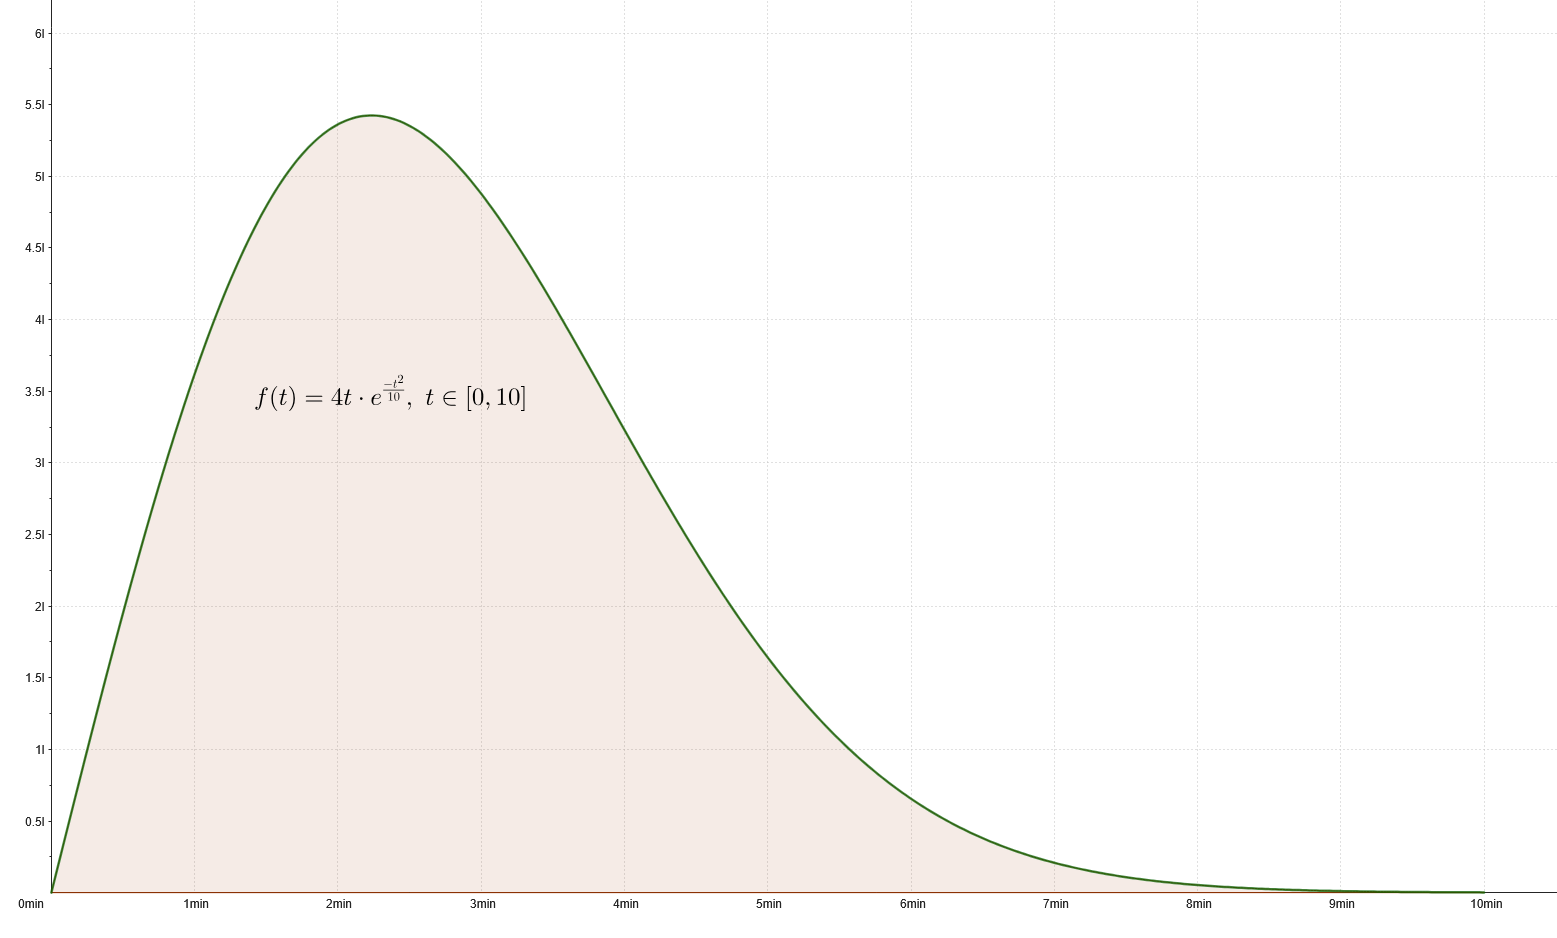
\includegraphics[scale=0.4]{2025-04-10_192739.png}
\end{center}
\oppgaveDel{c}
\begin{align*}
&\int_{0}^{10} f(x) dt = \int_{0}^{10} \left[ 4t \m e^{\frac{-t^2}{10}} \right] dt = \uuline{20} % TODO: LEGG TIL UTREGNING!!
%\left[ ??? \right]_{0}^{10}\\[0.2cm]
%& = ??? - 0 = \uuline{20}
\end{align*}
\oppgaveDel{d}
\begin{align*}
&\int_{0}^{5259600} f(x) dt = \int_{0}^{5259600} \left[ 4t \m e^{\frac{-t^2}{10}} \right] dt = \uuline{20} % TODO: LEGG TIL UTREGNING!!
\end{align*}
\oppgaveDelSlutt

% % % % % % % % % % % % % % % % % % % % % % % % % % % % % % % % % % % % % % % % 

\newpage
\oppgave{5}
\begin{align*}
&f(x) = \frac{1}{2}x\\
&g(x) = -x^2 + 5
\end{align*}
\oppgaveDelStart
\oppgaveDel{a}\ \\
\begin{center}
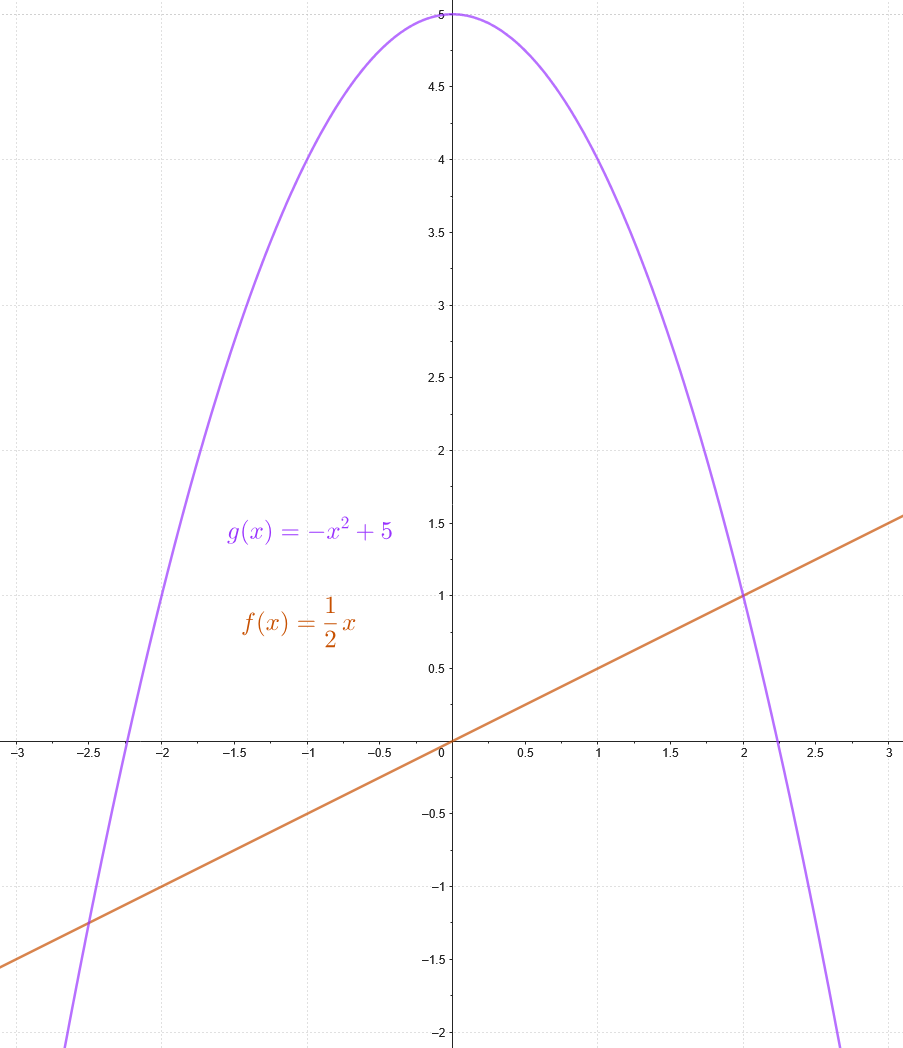
\includegraphics[scale=0.4]{2025-04-10_202031.png}
\end{center}
\oppgaveDel{b}
\begin{align*}
& \int_{0}^{2} f(x)dx = \int_{0}^{2} \left[ \frac{1}{2}x \right] dx = \left[ \frac{1}{2} \m \frac{1}{2} x^2 \right]_{0}^{2} = \left[ \frac{1}{4}x^2 \right]_{0}^{2} = \frac{1}{4} 2^2 - \frac{1}{4} 0^2 = \frac{4}{4} - 0 = \uuline{1}\\\\
& \int_{0}^{2} g(x)dx = \int_{0}^{2} \left[ -x^2 + 5 \right] dx = \left[ \frac{-x^3}{3} + 5x \right]_{0}^{2} = \left( \frac{-2^3}{3} + 5 \m 2 \right) - 0 = \frac{30}{3} - \frac{8}{3} = \uuline{\frac{22}{3}}
\end{align*}
\oppgaveDel{c}
\begin{align*}
&\text{Skjæringspunktene mellom $f(x)$ og $g(x)$ er:}\\[0.2cm]
&\frac{1}{2}x = -x^2 + 5\\[0.2cm]
&x^2 + \frac{1}{2} x - 5 = 0\\[0.2cm]
&\boxed{ax^2 + bx + c = 0} \rightarrow \boxed{x = \frac{-b \pm \sqrt{b^2 - 4ac}}{2a}}\\[0.2cm]
&a = 1,\ \ b = \frac{1}{2},\ \ c= -5\\[0.2cm]
&x = \frac{-\frac{1}{2} \pm \sqrt{(\frac{1}{2})^2 - 4 \m (-5))}}{2} = \left(- \frac{1}{2} \pm \frac{9}{2} \right) \m \frac{1}{2}\\[0.2cm]
&x = \frac{-10}{2} = - 2,5\ \ \ \lor\ \ \ x = \frac{8}{2} = 2\\\\
&\text{$f(x)$, $g(x)$ og linjen $x = 0$ danner to arealer. Et på venstresiden av origo med $x$-verdi}\\
&\text{fra $-2,5$ til 0, og et annet areal på høyresiden av origo med $x$-verdi fra $0$ til $2$.}\\\\
&\text{Arealet på venstresiden er:}\\[0.2cm]
&\int_{-2,5}^{0} \left[ g(x) - f(x) \right] dx = \left[ \frac{-x^3}{3} + 5x - \frac{x^2}{4} \right]_{-2,5}^{0}\\[0.2cm]
&= 0 - \left( - \frac{(-2,5)^3}{3} - \frac{(-2,5)^2}{4} + 5 \m (-2,5) \right) = \uuline{8,85}\\\\
&\text{Arealet på høyresiden er:}\\[0.2cm]
&\int_{0}^{2} \left[ g(x) - f(x) \right] dx = \left[ \frac{-x^3}{3} + 5x - \frac{x^2}{4} \right]_{0}^{2}\\[0.2cm]
&= - \frac{2^3}{3} - \frac{2^2}{4} + 5 \m 2 = \frac{22}{3} - \frac{3}{3} = \frac{19}{3} = \uuline{6,33}
\end{align*}
\oppgaveDelSlutt

% % % % % % % % % % % % % % % % % % % % % % % % % % % % % % % % % % % % % % % % 

\end{document}
